\section{Quantified World}
\subsection{Objects and subjects}
Following the age old approach to reality of natural philosophy to distinguish between the observer and the observed world, I'd like to start this treatise with an attempt of an abstraction what it means to be an observer and what it means to be observed.\\
It is an intrinsic property of an abstraction to focus on a limited set of properties, such that it allows to build a model in an attempt to describe the observed reality by reducing it to the chosen abstraction. The following pages are no different.\\

I'm postulating the object's existence and its state to be independent of any observer.
Doing otherwise would imply an unknown synchronization mechanism between multiple observers in order to obtain consistent observations. Assuming the object's independent existence seems simpler in comparison.
\begin{axiom}
Objects exist independently of any observer.
\end{axiom}
\begin{definition}
\marginpar{Quantification of the extracted information?}
A measurement $\hat{q}$ is a means of an observer to extract information from its environment $\Psi$. The extracted information takes the form of an arbitrarily long series of observations\footnote{In most cases represented by a real number $\mathbb{R}$.}.
\end{definition}
In the limit of infinite many observations, a measurement $\hat{q}$ leads to a probability density of observations:
\begin{equation}
\hat{q}(\Psi)\equiv P(\Psi\rvert q)dq\quad.
\end{equation}
\begin{definition}
The observed environment $\Psi$ consists of an object in a specific state $\Psi_0$, if $\hat{q}(\Psi)$ has a single global and local maximum.
\end{definition}
\begin{definition}
An object is a succession of states $\Psi_\tau$ for which $P(\Psi_\tau\rvert q_j)$ has a single global and local maximum for all $\tau\in I\subset\mathbb{R}$ and all measurements $q_j$. $I$ is the lifetime of the object.
\end{definition}
\begin{equation}
\hat{q}(\Psi_\tau)=P(\Psi_\tau\rvert q)dq=P(\Psi_0\rvert f_\tau(q))dq=\int dq' P(\Psi_0\rvert q')u_\tau(q',q)dq
\end{equation}
\begin{equation}
\hat{q}(\Psi_\tau)=P(\Psi_\tau\rvert q)dq=P(\Psi_0\rvert f_\tau(q))dq=\int dq' P(\Psi_0\rvert q')\frac{\partial q}{\partial q'}(q';\tau)
\end{equation}
\begin{equation}
\int dq\int dq' P(\Psi_0\rvert q')u_\tau(q',q) = 1\qquad\forall P(\Psi_0\rvert q')
\end{equation}
\begin{subequations}
\begin{eqnarray}
\int dq' u_\tau(q_2,q')u_\tau(u',u_1)\equiv\delta(q_2,q_1)\\
u_\tau(q_2,q_1)^{-1}= u_\tau(q_1,q_2)= u_{-\tau}(q_2,q_1)\\
\lim_{\tau\rightarrow 0}u_\tau(q_2,q_1)=\delta(q_2,q_1)
\end{eqnarray}
\end{subequations}
The concept of an object relies on the existence of a subset of measurements which remain whose results are continuous in the moments of subsequent observations. This existence of continuity is crucial for the observer in order to identify a series of observations with different states of the same object. What happens to the object in between two observations is of no concern to the observer\footnote{See \href{https://en.wikipedia.org/wiki/Ship_of_Theseus}{Ship of Theseus}.}.\\
A measurement of a state results therefore in a probability distribution of multiple independent observations performed by one or more observers with identical sensors on one or more objects in the same state $\Psi$.
In this sense I define an observer\footnote{Some schools of philosophies use the term \href{https://en.wikipedia.org/wiki/Subject_(philosophy)}{subject}.} as a set $\hat{q}\equiv\{q_j\}$ of possible measurements.\\
An observation is the result of a single interaction of the observer with the object.
A measurement is the probability distribution of expected observations obtain as the asymptotic limit of arbitrarily many independent observations of the same object.
A property of an object is a measurement with a single most probable observation over all open subsets in the space of observed values (no competing local maxima).
An observer, equipped with the equipment to perform a measurement $\hat{q}$ on an object in state $\Psi$, obtains a set of observed values $q\equiv\{q_j\}$. The probability distribution $\hat{q}(\Psi)$ of those observations constitutes the most complete description of $\Psi$ with the measurements at the observer's disposal.
If a measurement doesn't have a single global and local maximum, the observed state doesn't belong to one object, but might be an indications that multiple distinct objects are being observed.
\begin{figure}[ht]
\centering
\begin{tabular}{cc}
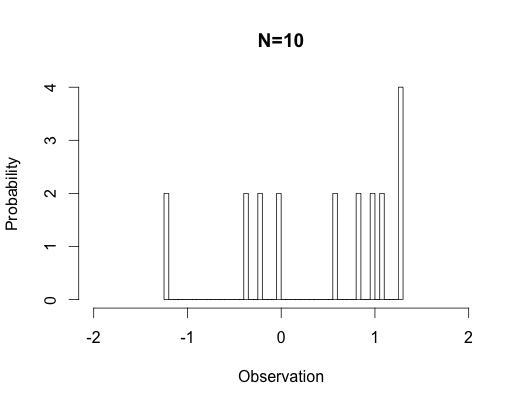
\includegraphics[width=0.5\textwidth,trim={0 20 50 0},clip]
{img/StateComposition_10.png}&
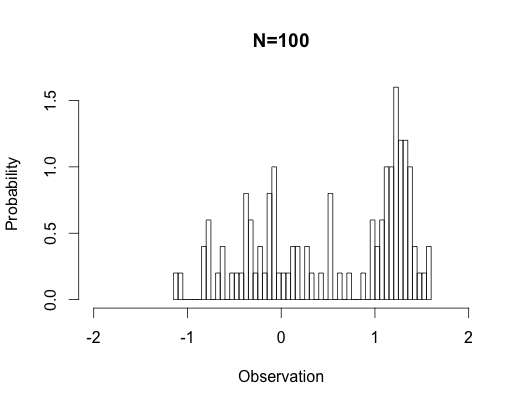
\includegraphics[width=0.5\textwidth,trim={0 20 50 0},clip]{img/StateComposition_100.png}\\
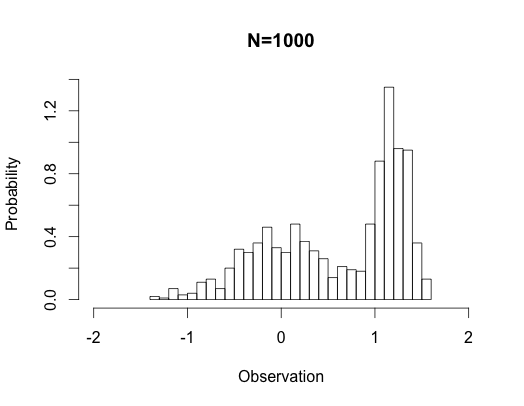
\includegraphics[width=0.5\textwidth,trim={0 20 50 0},clip]{img/StateComposition_1000.png}&
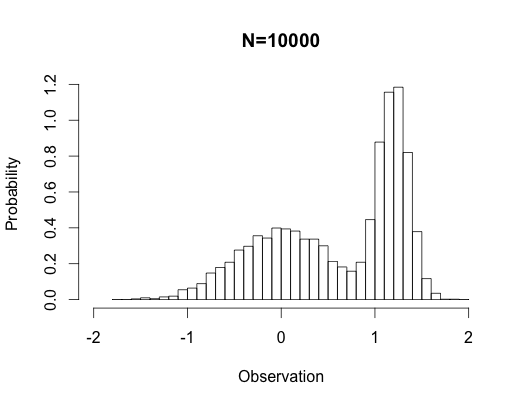
\includegraphics[width=0.5\textwidth,trim={0 20 50 0},clip]{img/StateComposition_10000.png}
\end{tabular}
\caption{Measurements on a composite object with increasing number $N$ of observations.}
\label{figQuoteChangeCluster}
\end{figure}
\begin{theorem}
Here is a new definition
\begin{proof}
Here is my proof
\end{proof}
\begin{example}
asd
\end{example}
\begin{example}
asd
\end{example}
\end{theorem}
The dualism between object and observer doesn't allow independent definitions of these two concepts. Instead both concepts are related to measurements and observations. of an object and an observer are 
Note that the term $\mathcal{O}(\Phi)$ implies the assumption that an object $\Phi$ has an existence independent  of the observer $\mathcal{O}$. Different observers might perform different measurements of the same object.


The distinction and interaction between the observable universe and the observer is a traditional topic for philosophical discourses. Physics as a natural philosophical discipline makes no exception. We start this overview of my understanding of the mathematical description of the world's behaviour therefore with the definition of a physical object:\\
A physical object is identified with a complete description of the physical object.
The description of a physical object is complete if it contains the results of all possible measurements of the physical object in question.\\
Since the topic of this treatise is an overview of the physical world, the term "object" are always to be understood as "physical object".\\
This definition provokes the question: What is a measurement?
 

A subject is an observer and an object is a thing observed. An object is a set of properties, i.e. measurements. A property consists of a measurement on an object and its result. An red apple is an object for which the measurement of its color results in red.
\subsection{Measurements}
A measurement of an object's property results in a probability distribution for the outcome of an single observation.
Measurements enable an observer to relate different objects by comparison. A property of an object is only meaningful if it can be compared to the same property of another object. E.g.: The property ”color” is only meaningful if there exist other objects with different values of this property. Saying an apple has the property ”rupalsy” of (let’s say) 5 is meaningless unless we find other objects on which the measurement of ”rupalsy” reveals this specific property of the objects in question.\\
Length, mass, time intervals, electrical charge are examples of measurements. But also volume, temperature, torque etc.\\
Since an object is defined by its properties, each the result of a measurement, an object can be represented as an element of the space of all measurement results: the state space of the object.
Calling an object’s properties the state of an object implies a possible transition from one set of properties to another with an equivalency of these two states by attributing them to the same object. I.e. even if an oven changes its temperature, its still the same oven.\\
\begin{tabular}{| l | c | c | c |}
\hline
\multicolumn{4}{| c |}{Mechanics}\\
\hline
$F_1$ & $F_1(q,Q,t)$ & $p=-\frac{\partial F_1}{\partial q}$ & $P=\frac{\partial F_1}{\partial Q}$\\
$F_2$ & $F_2(q,P,t)=F_1-QP$ & $p=-\frac{\partial F_2}{\partial q}$ & $Q=-\frac{\partial F_2}{\partial P}$\\
$F_3$ & $F_3(p,Q,t)=F_1+qp$ & $q=\frac{\partial F_3}{\partial p}$ & $P=\frac{\partial F_3}{\partial Q}$\\
$F_4$ & $F_4(p,P,t)=F_1+qp-QP$ & $q=\frac{\partial F_4}{\partial p}$ & $Q=-\frac{\partial F_4}{\partial P}$\\
\hline
\hline
\multicolumn{4}{| c |}{Thermodynamic potentials}\\
\hline
Internal energy& $U(V,S,t)$ & $p=-\frac{\partial U}{\partial V}$ & $T=\frac{\partial U}{\partial S}$ \\
Helmholtz free energy& $A(V,T,t)=U-ST$ & $p=-\frac{\partial A}{\partial V}$ & $S=-\frac{\partial A}{\partial T}$\\
Enthalpy& $H(p,S,t)=U+pV$ & $V=\frac{\partial H}{\partial p}$ & $T=\frac{\partial H}{\partial S}$\\
Gibbs free energy& $G(p,T,t)=U+pV-ST$ & $V=\frac{\partial G}{\partial p}$ & $S=-\frac{\partial G}{\partial T}$\\
\hline
\end{tabular}\\
\begin{definition}
The configuration space $\mathcal{C}$ of a physical object consists of all physical states accessible to this object. Let $q$ be a set of coordinates on $\mathcal{C}$.
\end{definition}
\begin{axiom}
In order to be continuously recognizable by the observer as the same physical object, any evolution of a physical state $\Psi_0$ of the object occurs along a continuous path $\left\{\Psi_\tau\rvert\tau\in\mathbb{R}\right\}\subset\mathcal{C}$.
\end{axiom}
\begin{definition}
The path $\left\{\Psi_\tau\rvert\tau\in\mathbb{R}\right\}\subset\mathcal{C}$ is the object's history.
\end{definition}
\begin{axiom}
\marginpar{Does this prohibit some histories on $\mathcal{C}$?}
An object's history locally minimizes the path integral of a Lagrangian 1-form $L(q,\dot{q})d\tau$ on $\mathcal{C}$.
\end{axiom}
\begin{definition}
The action $S$ is the value of the path integral between two states in an object's history.
\begin{equation}
S(q_1,q_0;\tau_1-\tau_0) \equiv \int_{\tau_0}^{\tau_1}d\tau L(q,\dot{q})\quad.
\end{equation}
\end{definition}
\begin{theorem}
Two states $\Psi_{\tau_0}$ and $\Psi_{\tau_1}$ from the object's history and a Lagrangian 1-form $L(q,\dot{q})d\tau$ on $\mathcal{C}$ determine all the intermediate states.
\begin{proof}
Let $\delta q(\tau)$ be a path variation which leaves the end points $q_0\equiv q(\Psi_{\tau_0})$ and $q_1\equiv q(\Psi_{\tau_1})$ invariant, i.e. $\delta q(\tau_{0})=\delta q(\tau_{1})\equiv 0$.
\begin{equation}
\begin{split}
0&=\delta\int_{\tau_0}^{\tau_1}d\tau L(q,\dot{q})=\int_{\tau_0}^{\tau_1}d\tau\sum_j\left\{\frac{\partial L}{\partial q_j}\delta q_j+\frac{\partial L}{\partial \dot{q}_j}\delta\dot{q}_j\right\}\\
&=\int_{\tau_0}^{\tau_1}d\tau\sum_j\left\{\frac{\partial L}{\partial q_j}\delta q_j+\frac{d}{d\tau}\left[\frac{\partial L}{\partial\dot{q}_j}\delta q_j\right]-\frac{d}{d\tau}\frac{\partial L}{\partial \dot{q}_j}\delta q_j\right\}\\
&=\int_{\tau_0}^{\tau_1}d\tau\sum_j\left\{\frac{\partial L}{\partial q_j}-\frac{d}{d\tau}\frac{\partial L}{\partial \dot{q}_j}\right\}\delta q_j+\left[\frac{\partial L}{\partial\dot{q}_j}\delta q_j\right]_{\tau_0}^{\tau_1}\nonumber
\end{split}
\end{equation}
\marginpar{Does this imply a unique history?}
Since this condition is supposed to hold for all possible path variations, the path is locally given by
\begin{equation}
\frac{d}{d\tau}\frac{\partial L}{\partial \dot{q}_j}-\frac{\partial L}{\partial q_j}=0\qquad \forall j\quad.
\end{equation}
\end{proof}
\begin{example}
Harmonic oscillator in 1 dimension\\
The Lagrangrian of a harmonic oscillator with mass $m$ and angular frequency $\omega$ is
\begin{equation}
L(q,\dot{q}) = \frac{m}{2}\dot{q}^2-\frac{m\omega^2}{2}q^2\quad.\nonumber
\end{equation}
The object's history is defined by the equation
\begin{equation}
\frac{d}{d\tau}\frac{\partial L}{\partial \dot{q}}-\frac{\partial L}{\partial q} = m\ddot{q}+m\omega^2q=0\quad.\nonumber
\end{equation}
\end{example}
\end{theorem}
\begin{definition}
The canonical momentum of $q_j$ is $p^j\equiv\frac{\partial L}{\partial\dot{q_j}}(q,\dot{q})$\quad.\\
\end{definition}
\begin{theorem}
Here is a new definition
\begin{proof}
Here is my proof
\end{proof}
\begin{example}
asd
\end{example}
\begin{example}
asd
\end{example}
\end{theorem}
\begin{theorem}
Here is a new definition
\begin{proof}
Here is my proof
\end{proof}
\begin{example}
asd
\end{example}
\begin{example}
asd
\end{example}
\end{theorem}